\chapter{Experiential Learning\\ of Networking Technologies}
\vskip -15pt

\centerline{{\LARGE\sl Understanding TCP Flow Control and Congestion Control}}

\vskip 0.8cm

\begin{center}
{\large\uppercase{Ram P. Rustagi}}, 

\vskip -6pt

Department of CSE, KSIT Bengaluru 


\bigskip
{\large\uppercase{Viraj Kumar,}} 

\vskip -6pt

Divecha Centre for Climate Change, IISc Bengaluru

\end{center}

\vskip 2.3cm



\vfill


%~ \noindent\makebox[\textwidth]{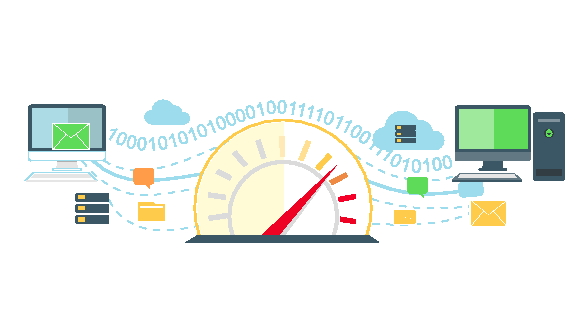
\includegraphics[width=1.05\paperwidth,height=13cm]{src/Figures/chap5.jpg}}
%~ \begin{textblock}{16}(0,8.815)
%~ \noindent\centerimg[width=\paperwidth]{src/Figures/chap5.jpg}
%~ \end{textblock}
\newpage

\begin{multicols}{2}

\section*{Abstract} 

In a TCP connection, the underlying network drops packets when it lacks the capacity to deliver all the packets sent by the sender to the receiver. This phenomenon is called congestion. TCP at the sender’s side will not receive \textit{acks} for these dropped packets. Since TCP is a reliable protocol, the sender must retransmit all these packets. The mechanism used by TCP to deal with such situations is called TCP Congestion Control. In this article, we explain the basics of congestion control and provide experiential exercises to help understand its impact on TCP performance.

\section*{Introduction}

We discussed TCP flow control in our previous article \cite{art2-key01}, and we saw that the receiver controls the rate at which the sender can send the data. To achieve this, the receiver informs the sender about its available buffer size (which may be dynamically adjusted), and the sender restricts the transmission of data so that it does not exceed this buffer size. This flow control feature is \textit{independent} of the network capacity – it is \textit{entirely} controlled by the buffer size available at the receiver. If the underlying network’s capacity is greater than the data rate controlled by TCP flow control, then TCP throughput simply depends upon flow control. However, in today’s environment, both the server and client hardware have enough memory available to allow their buffer sizes to be up to 1 GB (the maximum value for flow control supported by TCP). Thus, flow control rarely has an impact on TCP performance, except where memory is a severe constraint e.g., with IoT (Internet of Things) devices in certain instances.

In general, a bigger challenge in attaining high TCP performance is determining the optimal rate at which a server can transmit data to the client. Since TCP \cite{art2-key02} is an end-to-end protocol, this optimal rate is not known at the time when the client connects to the server. Further, this optimal rate can vary significantly – the unpredictable nature of packet arrivals will inevitably place high traffic on certain links at some time, but lower traffic at other times. The mechanism used by the server to discover this optimal transmission rate is called Congestion Control.

Clearly, if the server sends data at a rate lower than the capacity available in the network, it will be under-utilizing the network and it will take longer than necessary to transmit the data. On the other hand, if the server tries to send data at an excessively high rate, the network will choke. More precisely, packets will start to queue at buffers of intermediate network devices. If these buffers become full, any additional packets will be dropped as per the queuing policy (Random Early Detection, Fair Queuing, Weighted Fair Queuing, etc.). At this point, or perhaps even sooner, the sender will fail to receive acknowledgements for packets it had sent (either due to packet drop or timeout), and the sender will be forced to retransmit data packets. These duplicate packets can easily lead to further network delays. Hence, to achieve high performance, it is crucial that the mechanism for Congestion Control adapts rapidly. In reality, this is a complex and challenging task.

\section*{Basis of TCP Congestion Control}

Both Flow Control and Congestion Control seek to improve TCP performance. They are inter-related, and they both deal with errors (packets lost/corrupted/discarded) by retransmitting these packets. It is tempting to view these two behaviors as synonymous, but it is important to understand that they are different. At a high level, TCP tries to deliver optimal performance by:
\begin{itemize}
\item[i.] Sending only as much data as can be received by a receiver i.e., data which can be transmitted by the sender without waiting for the \textit{ack}, and should not exceed the receiver’s buffer size. This is dealt with by TCP Flow Control.
\item[ii.]  Dynamically adjusting the rate at which the sender transmits data to match the network’s ever-changing capacity. This is dealt with by TCP Congestion Control.
\end{itemize}

It should be intuitively clear that it is essentially impossible to predict the available network capacity ahead of time with reasonable accuracy, given that vast numbers of users are making autonomous decisions that lead to TCP connections and data transfer between clients and servers. In the absence of a good prediction, we use the network capacity in the recent past as the best available estimate of the capacity in the immediate future. Thus, TCP congestion control works by probing the network capacity and adjusting the sender’s transmission rate based upon the probe result. This probing is implicit – there is no explicit probe message. Instead, each data transmission and its \textit{ack} (or even the absence of an \textit{ack}) is used as a probe to estimate network capacity.

In the initial phase of TCP connection and data transfer, early TCP implementations followed a mechanism called \textit{Slow Start}. After a TCP connection is established using a 3-way handshake  \cite{art2-key02}, the sender sends one data segment (also known as a congestion window of size 1, or \textit{cwnd} = 1). If it receives the acknowledgement in expected time, it deduces that the network is fine. Then, it repeatedly increases the transmission rate by doubling the congestion window size \textit{cwnd} each time it receives \textit{acks} for all segments within the expected time.

At some point, this exponential growth in transmission rate will exceed the network’s capacity. When some of these segments are lost (or delayed so much that these are considered equivalent to lost), the TCP stack at the receiver will continue to send \textit{acks} for any new data segment it receives out of order. Note such an \textit{ack} will acknowledge only the last segment it received in order, and not the segment it received out of order. This is because TCP is a streaming protocol, so any acknowledgement implies that all the data bytes up to this acknowledgement value have been received. To better understand this point, suppose the sender is sending data in segments of size of 1000 bytes each. The acknowledgement number indicates the offset of the next byte (in the continuous stream of data) that the receiver is expecting in the next data segment. Thus, when receiver receives first 1000-byte segment, the acknowledgement number will be 1001. In general, the acknowledgement for the $N^{\rm th}$ segment will be $1000N + 1$. Now, suppose that the sender has transmitted segments $N-2$, $N-1$, $N$ and $N+1$ and the network loses the \textit{ack} for segment $N-2$ (from receiver to sender after receiving segment $N-2$) and the entire segment $N$ (from sender to receiver). Assume that the network loses no other packets. Thanks to the cumulative acknowledgement\footnote{There are implementations of TCP that follow selective ack rather than cumulative ack, where each packet must  be individually \textit{acked}.} policy followed by TCP, when the sender receives the \textit{ack} for segment $N-1$ (whose acknowledgement number is $1000(N-1) + 1$), it knows that the receiver successfully received segment $N-2$. It can also infer that there may have been some congestion in the network that cause the ack for segment $N-2$ to be dropped, but this seems to have cleared up (since the \textit{ack} for segment $N-1$ was successfully received). After segment $N$ is lost, if the receiver gets segment $N+1$ it will respond with the acknowledgement number $1000(N-1) + 1$ once again, indicating that it is still awaiting the first byte of segment $N$. (The TCP standard RFC 793 \cite{art2-key02} does not specify whether the receiver should discard the segment $N+1$ that was received out-of-order, or store it for future use.) When the sender receives this duplicate \textit{ack}, it can again infer that there is congestion in the network. If the receiver now receives segments $N+2$, $N+3, … $ etc. without receiving segment $N$, the \textit{acks} it responds with for these segments will again have the acknowledgement number $1000(N-1) + 1$. The server can infer that network may have mild congestion, and it can slow down the data transmission rate to avoid aggravating the problem. On the other hand, if the server fails to receive any ack beyond $1000(N-1) + 1$, it can infer that the network is witnessing serious congestion. In this case, the sender will slow the transmission to the lowest possible rate to help network to recover from congestion. TCP has several different implementations, such as TCP Tahoe, TCP Reno, TCP Vegas, etc. which primarily differ in the way they treat congestion. The focus of this article is to understand the core behaviour of TCP, as well as a few other relevant characteristics such as TCP fairness. 

\section*{TCP Congestion Management Principles}

The primary mechanism for congestion management adopted by the TCP protocol is to continuously adjust the sender’s transmission rate so as to optimally use the underlying network. Essentially, the sender should try to send data at the highest rate possible without causing congestion in the network. This becomes particularly important when the underlying network’s capacity keeps on changing continuously on account of network usages by other Internet hosts. Further, the only information available to a TCP sender is how many data segments it has sent, which acknowledgements have been received, and the occurrence of timeouts (i.e., failure to receive acknowledgements within expected time). A TCP sender has no knowledge of how many other senders are using the network and what their transmission rates are. TCP makes use of the following criteria to achieve its optimal transmission rate. For a detailed discussion of these criteria, reader should refer to  \cite{art2-key03}.
\begin{itemize}

\itemsep=.2cm

\item[i.] \textit{Lost segment:} When a segment is lost (when an \textit{ack} is not received within the expected time or when duplicate \textit{acks} are received for earlier segments), it implies some network congestion and thus the sender should decrease its transmission rate.
\item[ii.] \textit{Acknowledgement receipt:} A fresh \textit{ack} (not a duplicate one) for a data segment implies that there is no network congestion at present. A duplicate \textit{ack} implies that the network had some disturbance in the past, but it now seems to have recovered from it – as of now there is no congestion but any increase in traffic might lead to congestion again.
\item[iii.] \textit{Probing of the available bandwidth:} To achieve optimal use of available network bandwidth, TCP follows the strategy of increasing the transmission rate when an ack is received and decreasing the transmission rate when it perceives that its transmitted segment is lost.
\end{itemize}

Using these criteria, Van Jacobson described TCP Congestion Avoidance and Control \cite{art2-key04} in 1998, and further along all the parts of the intertwined congestion control algorithms are summarized in RFC 5681  \cite{art2-key05}.  The TCP Congestion Control algorithm primarily consists of 3 phases, namely
\begin{itemize}
\item[i)] Slow Start phase,

\item[ii)] Congestion Avoidance phase, and

\item[iii)] Fast Recovery phase. 
\end{itemize}

The difference among these various congestion control algorithms are on account of how these 3 phases are intertwined together. We will briefly discuss all these 3 phases and define experiments to imbibe the experiential learning of the same.

TCP is a streaming protocol \cite{art2-key13} and does not honour any message boundary i.e., the receiver never knows how many segments the sender has sent – it only sees a stream of bytes. For simplicity of understanding, we will consider TCP segments in terms of TCP MSS (Max Segment Size)-\cite{art2-key06}\cite{art2-key07}, which on an Ethernet LAN link corresponds to 1460 bytes. Thus, for the description below, segments and acks will be referred to in terms of MSS. Further, the only way TCP can detect packet loss is if the sender times out before receiving an ack. We will refer to this timeout in terms of Round-Trip Time RTT, which correspond to the difference between the time when a sender starts transmitting a segment and the time when it receives its acknowledgement. We also formally define the congestion window (\textit{cwnd}) as the number of TCP segments that can be sent one after the other without waiting for an \textit{ack}. Thus, if there is no congestion in the network, a high value of \textit{cwnd} implies that many segments can be transmitted one after the other, resulting in better throughput for the TCP connection.

\setcounter{figure}{0}
\begin{figure}[H]
\centering
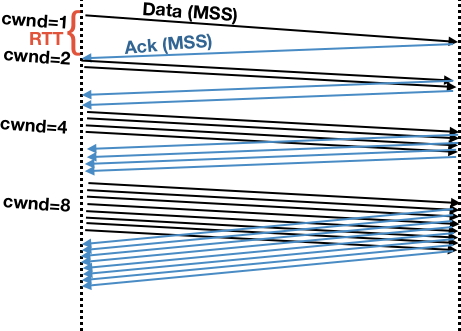
\includegraphics[scale=2.1]{src/Figures/chap2/chap2-fig01.jpg}
\caption{TCP Slow start}\label{chap2-fig01}
\end{figure}

When a TCP connection is setup using 3-way handshake, the time duration between SYN sent and SYN-Ack received is used to compute the first RTT. Using this RTT value, and taking into account some variation, an estimated timeout for receiving the \textit{ack} for the next transmitted segment is computed  \cite{art2-key03}. Thus, when the 3-way handshake completes, the sender can estimate the RTT but it does not have any information about the network capacity. Thus, data transmission on this connection starts with \textit{cwnd} conservatively set to 1. When the \textit{ack} for \textit{cwnd}=1 is received within the estimated timeout, \textit{cwnd} is doubled and increased to 2 (the sender transmits 2 segments one followed by the other). When the ack for \textit{cwnd}=2 is received, \textit{cwnd} value is doubled and set to 4, and the sender transmits 4 segments one after the other. This doubling phenomenon is shown in Figure~\ref{chap2-fig01}.

Despite the exponential growth in transmission rate, this phase is called Slow start because of the conservative initial value \textit{cwnd}=1. The doubling of \textit{cwnd} can actually be accomplished more efficiently than shown in Figure~\ref{chap2-fig01}. To understand this, suppose \textit{cwnd}=4 i.e., the sender has transmitted 4 segments. One naïve choice would be to wait for all 4 \textit{acks} before doubling \textit{cwnd} to 8. Instead, it is more efficient to increase \textit{cwnd} by 1 each time an \textit{ack} is received: when the first of the 4 \textit{acks} is received \textit{cwnd} becomes 5, when the second \textit{ack} is received \textit{cwnd} becomes 6, etc. When the fourth \textit{ack} is received \textit{cwnd} becomes 8 as shown in Figure~\ref{chap2-fig02}.

\begin{figure}[H]
\centering
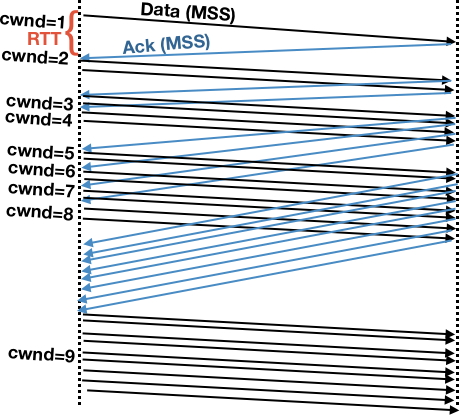
\includegraphics[scale=2]{src/Figures/chap2/chap2-fig02.jpg}
\caption{Slow Start phase- doubling of cwnd (incrementing it with each ack) and using ssthreshold=8}\label{chap2-fig02}
\end{figure}

It is important to restrict this exponential growth below a limit in order to avoid severe congestion. This limit is called \textit{ssthreshold} (slow start threshold). The setting of the initial value depends upon the TCP stack implementation. For example, \textit{ssthreshold} is 10 for Ubuntu (16.04 LTS). Figure~\ref{chap2-fig03} shows the growth of \textit{cwnd} in slow start phase with initial value of \textit{sshthreshold} as 20. In this figure, the X-axis corresponds to time and the Y-axis corresponds to \textit{cwnd} value. The first round-trip time is about 200ms (actual value: 0.21296s) and \textit{cwnd} starts from value 1 at time T=0s. At time T=0.2s (first RTT), \textit{cwnd} becomes 2. At time T=0.4s (second RTT), \textit{cwnd} becomes 4, and at third RTT (time T=0.66s), \textit{cwnd} becomes 8, and at time T=0.92s (fourth RTT), \textit{cwnd} becomes 16. The exponential growth stops when \textit{cwnd} reaches the slow start threshold (ssthreshold) value of 20 at time 1.08s. 

\begin{figure}[H]
\centering
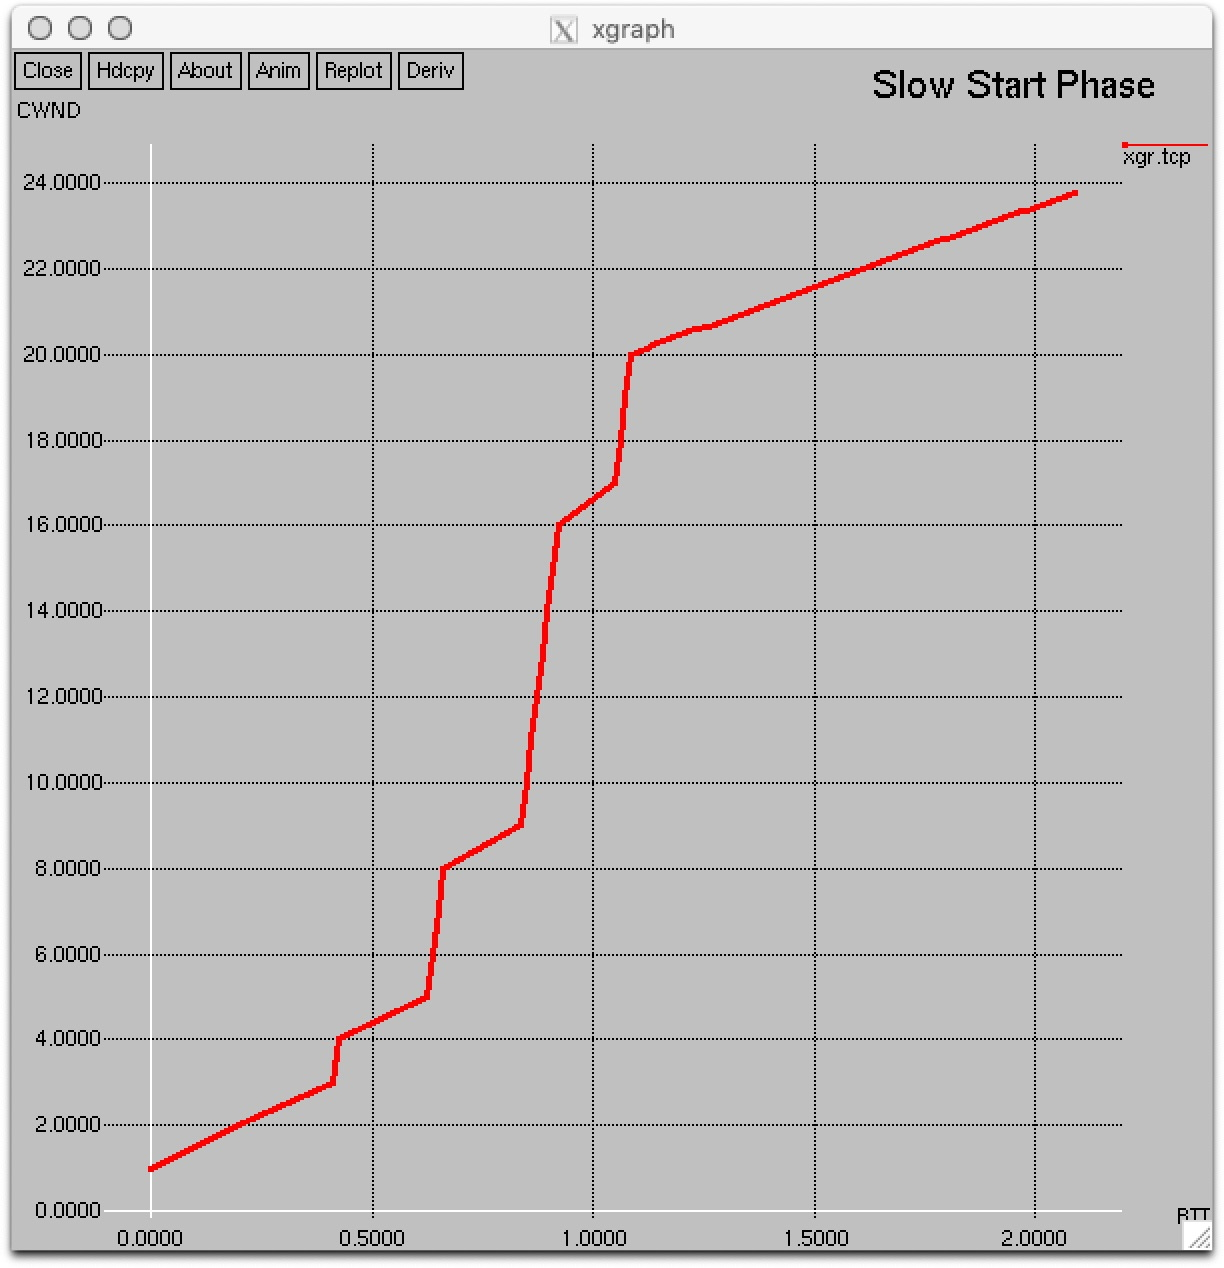
\includegraphics[scale=.87]{src/Figures/chap2/chap2-fig03.jpg}
\caption{Growth of congestion window in Slow Start phase}\label{chap2-fig03}
\end{figure}

The current TCP implementation of operating systems such as Windows, Linux, Mac are optimized, and it may not be easy for the reader to play with TCP tuning parameters to achieve the exact behavior as shown in the graph. The TCP congestion control mechanism followed by Ubuntu Linux is called Cubic \cite{art2-key08} where rather than starting from \textit{cwnd}=1, it simply starts with a higher value depending upon network bandwidth and round-trip time. Thus, to understand the basic TCP slow start phase, an experiment is conducted using NS2 simulator \cite{art2-key09}. Details of installing NS2 and associated tools such as Network Animator (nam) \cite{art2-key10} and Xgraph\cite{art2-key11}, are given in the Appendix. To develop a better understanding of the slow start phase experimentally, the reader is requested follow the steps described in Exercise~\ref{chap2-exe01} by configuring desired values of \textit{ssthreshold}, and to plot the graph to study the exponential growth of \textit{cwnd}.

Naturally, an excessively high value of \textit{ssthreshold} can cause congestion and packet loss. Thus, when congestion occurs during the slow start phase (i.e., the sender does not receive acknowledgements for packets it has sent), the sender realizes that network is congested and starts over again with \textit{cwnd}=1.

\section*{Congestion Avoidance phase}

When \textit{cwnd} value reaches \textit{ssthreshold}, it increases the congestion window \textit{cwnd} slowly to avoid possible congestion. In this phase, \textit{cwnd} is increased by 1 when all the previous segments have been acknowledged. This is shown in Figure~\ref{chap2-fig02}  where when \textit{sshthreshold}=8, and after all the acks corresponding to all the 8 transmitted segments are received, \textit{cwnd} is increased by 1 and becomes 9. Similarly, in Figure~\ref{chap2-fig03}, \textit{ssthreshold} is set to 20, and thus after \textit{cwnd} becomes 20 at time T=1.08s, it increases linearly with each RTT. The Exercise~\ref{chap2-exe01} described the steps; to experimentally study the linear behaviour of \textit{cwnd} with different value of \textit{ssthreshold} after the former crosses \textit{ssthreshold} value. Thus, at time T=1.35s, \textit{cwnd} becomes 21, and at time T=1.62s, \textit{cwnd} becomes 22 and so on. The general efficient way to increase the \textit{cwnd} is not to wait for all the acks but rather increment the \textit{cwnd} value in such a way that it effectively increases by 1 MSS when all the acks are received. Thus, on each ack received, \textit{cwnd} is increased by \textit{MSS/cwnd} bytes. This is the approach followed in general by any current TCP implementation. The value of \textit{cwnd} will continue to increase linearly till either all the data is transmitted successfully or congestion is encountered When sender detects congestion (deduced, by loss of acknowledgements, it decreases the \textit{cwnd} to mitigate the congestion and thus enters the ${\rm 3}^{\text {rd}}$ phase of Fast Recovery. Exercise~\ref{chap2-exe02} describes the experimental set of steps to study the impact of initial value \textit{ssthreshold.}

\section*{Fast Recovery phase}

When TCP detects congestion, it differs in dealing with mild congestion and severe congestion to achieve optimal performance.  Mild congestion indicates that network witnessed some temporary disturbance and thus lost few packets but quickly recovered. Severe congestion indicates that network is still dealing with heavy traffic and losing all or most of the packets. In the early implementation of TCP (known as TCP Tahoe), it reacts strongly even for mild congestion and immediately brings down \textit{cwnd} to 1 and sets \textit{ssthreshold} to half of current \textit{cwnd} value. The \textit{cwnd}=1 reduces the traffic load by sender to the minimum to help the network recover from congestion at the earliest it is possible that network may have already recovered). Thus, TCP Tahoe does not differentiate between mild congestion and severe congestion The improved Implementation, TCP Reno, reacts differently to mild congestion and severe congestion. In both the cases, since some congestion has occurred it sets its \textit{ssthreshold} value to half of current \textit{cwnd} value. This helps in slow start phase as it cautiously probes the bandwidth linearly after reaching \textit{ssthreshold}. The primary thought behind decreasing \textit{ssthreshold} to half of the current \textit{cwnd} value is to help network recovery from congestion as well as to achieve a sustainable TCP throughput TCP Reno considers mild congestion as transient phenomenon and help quick recovery. When sender does not receive ack for $\text{N}^{\text{th}}$ segment, but  instead receives duplicate acks for $\text{(N-1)}^{\text{th}}$ segment, it deduces some congestion. When it receives 3 duplicate acks for $\text{(N-1)}^{\text{th}}$  segment, It considers that receiver hasn’t received $\text{N}^{\text{th}}$ segment (most likely it is lost and is unlikely to be delivered by network at all) but has received subsequent segments i.e. segments numbered N+1, N+2 and so on. This implies that mild congestion is over and sets this to half of current value i.e. sets \textit{cwnd=ssthreshold+3MSS} (increased by 1 for each of 3 duplicate ack received. Since, cwnd is not set to 1, but to an higher value it is treated as quick recovery from congestion and hence the name Fast Recovery phase.

The Figure~\ref{chap2-fig04} shows the transition between three phases of TCP congestion control. A detailed discussion of this state transition and how \textit{cwnd} is updated with each event is described in \cite{art2-key03}

\begin{figure}[H]
\centering
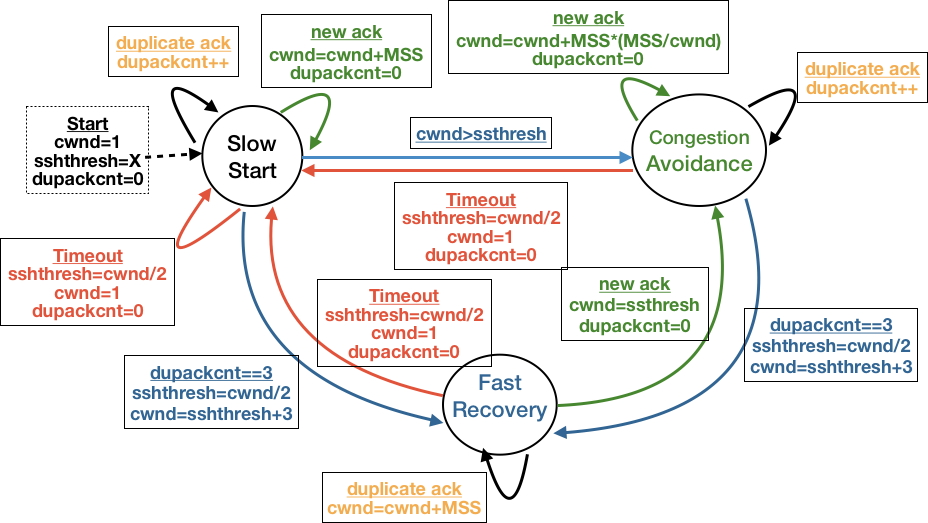
\includegraphics[scale=1.1]{src/Figures/chap2/chap2-fig04.jpg}
\caption{State Transition between different phases of congestion control}\label{chap2-fig04}
\end{figure}

\section*{Additive Increase Multiplicative Decrease (AIMD) behaviour}

The congestion control algorithm of a  TCP connection congestion control starts with Slow Start phase, and within few RTT cycles, \textit{cwnd} quickly  reaches the threshold limit \textit{ssthreshold} and enters Congestion Avoidance phase. In this phase, the TCP connection is likely to witness network congestion some time and thus it proceeds cautiously by (probing the network capacity) increasing \textit{cwnd} linearly by 1MSS when ack for all the transmitted segments are received. For simplicity assume that sender has enough data to send\footnote{By design, TCP performance is optimized for long duration connections.} and when \textit{cwnd} to reaches a value (even though with linear increase) greater than network capacity, it will experience network congestion causing loss of few transmitted packets. If network is still working and only few packets (corresponding to those that exceed network capacity) are lost, the sender will receive duplicate acks corresponding to segments having the acknowledge value corresponding to last received in order segment. As per TCP Reno congestion control implementation (or any similar variant), \textit{TCP} enters Fast Recovery phase after receiving 3 duplicate acks.  As \textit{cwnd} value is decreased by half, making it much lower than the estimated network capacity that was available when congestion occurred. As the transmitted load has decreased by half, It is expected that acks for newer transmitted segments will be received, and that is the reason TCP enters Congestion Avoidance Phase.  This transition from Congestion Avoidance Phase to Fast Recovery phase and back to Congestion Avoidance goes on forever till the sender transmits all the application data. This behaviour of \textit{cwnd} increasing linearly during congestion avoidance phase and then decreasing by half in  Fast recovery phase is shown in Figure~\ref{chap2-fig05}. The curve for \textit{cwnd} value looks like a saw tooth, and therefore TCP congestion control is also known as Additive Increase Multiplicative Decrease (AIMD) behaviour. This behaviour essentially demonstrates that TCP continues to probe for available bandwidth and adjusts its congestion window on continuous basis.

\begin{figure}[H]
\centering
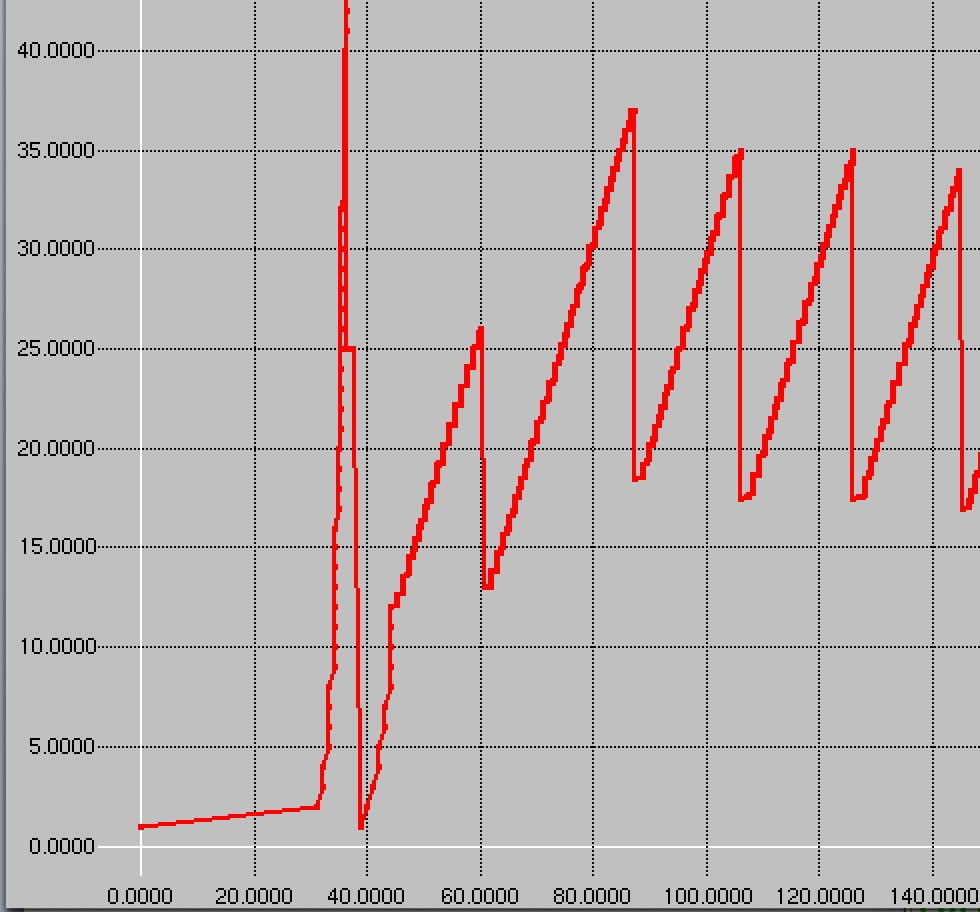
\includegraphics[scale=.96]{src/Figures/chap2/chap2-fig05.jpg}
\caption{Additive Increase Multiplicative Decrease}\label{chap2-fig05}
\end{figure}

After TCP Reno, a number of algorithms have been proposed and implemented to improve TCP congestion control, such as TCP Vegas,  TCP-BIC (Binary Increase Control), TCP-Cubic, TCP-Veno (combination of Vegas and Reno) etc. The default implementation in Linux OS is TCP-Cubic \cite{art2-key08}, where it starts with a higher value of \textit{cwnd} instead 1 and modifies the linear growth function to achieve more equitable bandwidth among many TCP connections that share the same network bandwidth. RFC 6928 \cite{art2-key07} suggests increasing the initial value of \textit{cwnd} and computed as min($10^{\ast}$MSS, max($2^{\ast}$MSS, 14600)). Exercise~\ref{chap2-exe03} describes the experiential exercise to study saw tooth behaviour.

\section*{TCP Fairness}

In real life, a TCP connection shares  some common link with other multiple TCP connections. Further, these TCP connections start at different point in time and terminate at different points in time.  Considering that all such connections are long-lived, and thus bandwidth of common link is shared among all the connections using the link. Thus, the question that arises is: \textit{“Does TCP treats fairly all the connections on a shared link”?}. At first thought, one would naturally think that the bandwidth of common link is shared on a first come first serve basis. This would imply that first such connection will consume almost full bandwidth and its \textit{cwnd} value will approximately correspond to shared link capacity and follow the saw tooth behaviour around this capacity. The value of \textit{cwnd} corresponding to subsequent connections using the shared link will mostly pertain to slow start phase, with underlying assumption being that these connections will see severe packet loss as maximum capacity is used by connections on first come first serve basis. However, it is interesting to study TCP fairness from a theoretical perspective as well as on empirical basis.

\begin{figure}[H]
\centering
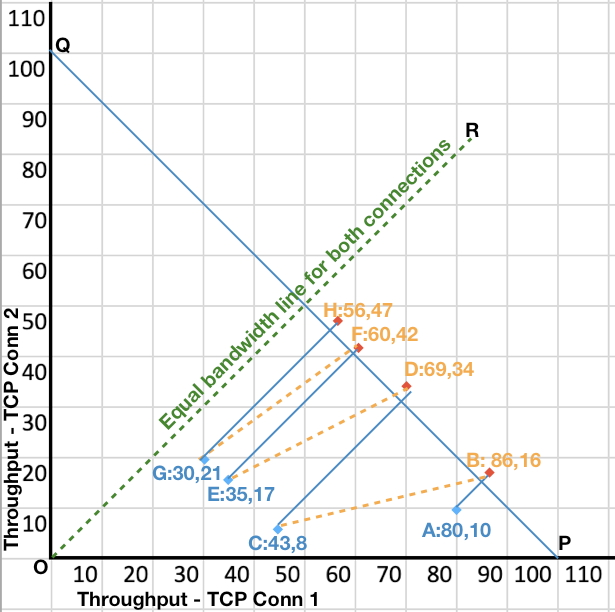
\includegraphics[scale=1.2]{src/Figures/chap2/chap2-fig06.jpg}
\caption{TCP Fairness}\label{chap2-fig06}
\end{figure}

For simplicity, consider that a network link has bandwidth of 100MSS, and is shared by two TCP connections Also, let us assume that ${\rm 2}^{\text{nd}}$ connection starts some time after the ${\rm 1}^{\text{st}}$  connection is established. Since connection 1 is established earlier, its \textit{cwnd} value will be much higher compared to \textit{cwnd} value of connection 2. The progress of \textit{cwnd} adjustment of these two connections is shown in Figure~\ref{chap2-fig06}. In any case, none of the individual connection can exceed the throughput  beyond 100MSS (max capacity of shared link). If connection 1 gets a full throughput of 100MSS, then connection 2 will get throughput of 0MSS (Point P) and vice versa (Point Q).  Line PQ defines the boundary of feasible throughput at any time. Any point on the line PQ or below corresponds to a feasible throughput and any point above the line PQ indicates congestion, which will lead to packet drop.

To understand the TCP fairness behaviour, consider that at some point in time, connection 1 is having \textit{cwnd}=80 and connection 2 is having \textit{cwnd}=10 as shown corresponding to point A in the Figure~\ref{chap2-fig06}. This is likely because saw tooth behaviour for connection 1 with vary its \textit{cwnd} between 50 (half of max throughput as when congestion occurs, \textit{cwnd} becomes half) and 100 (max throughput). At this point A, total \textit{cwnd} for both connections is 90 (=80+10) and which is less than 100 and thus no congestion would be seen. As both connections are in Congestion Avoidance phase and follow AIMD behaviour, \textit{cwnd} for both will increase linearly. For connection 1, it will progress thru \textit{cwnd}=81, 82, 83, 84 and 85 and similarly for connection 2, \textit{cwnd} will increase from 10 to 11, 12, 13, 14 and 15. The combined value of \textit{cwnd} becomes 100 MSS (equal to shared link capacity) and no congestion would be seen. At the next RTT cycle when all acks are received, \textit{cwnd} will become 86 for connection 1 and 16 for connection 2 (point B). This will result in network link getting a total traffic of 102MSS, exceeding its capacity of 100MSS. This will cause congestion and both connections will see packet drops and receive duplicate acks. As per AIMD behaviour \textit{cwnd} for both will decrease by half and will take the value \textit{cwnd}=43 for connection 1, and \textit{cwnd}=8 for connection 2 (point C). Since \textit{cwnd} has decreased and total cwnd now becomes 51 (=43+8), network will recover from congestion, and \textit{cwnd} for both connection 1 and 2 will start increasing linearly. Progressing in this way, connection 1 will have \textit{cwnd}=69, for and connection 2 will have \textit{cwnd}=34 (point D). This will cause, congestion to occur again, leading to packet drop and thus \textit{cwnd} will decrease by half resulting in \textit{cwnd}=35 for connection-1, and \textit{cwnd}=17 for connection-2 (point E). It will start increasing linearly again and will reach \textit{cwnd}=60 for connection-1 and \textit{cwnd}=42 for connection-2 (point F). At this point congestion would occur, decease the \textit{cwnd} by half for both (point G) and increase linearly again to have \textit{cwnd}=56 for connection-1 and \textit{cwnd}=47 for connection-2 (point H). After few such oscillations, both \textit{cwnds} will coincide and move along the line OR, which corresponds to using equal bandwidth for both connections. Thus, irrespective of whether a TCP connection starts early or later, TCP congestion control mechanism ensures that after some round of adjustments, \textit{cwnds} for all TCP connections will coincide with each other. This basically shows that TCP is always fair to all connections sharing a common link. However, it should be noted that the fairness of TCP is with respect to connections and not with respect to machines. For example consider a case where machine X is using N number of connections and machine Y is using M number of connections, and if the total bandwidth of the shared link for these M+N connections is R, then after some time, each connection will witness the saw tooth behaviour with its throughput varying between R/($2^{\ast}$(M+N)) and R/(M+N). If M is much larger than N, then machine X will get much larger share of bandwidth varying between $\text{M}^{\ast}$R/($2^{\ast}$(M+N)) and $\text{M}^\ast$R/(M+N) compared to machine Y having its share of bandwidth varying between $\text{N}^{\ast}$R/($2^{\ast}$(M+N)) and $\text{N}^{\ast}$R/(M+N).

\begin{figure}[H]
\centering
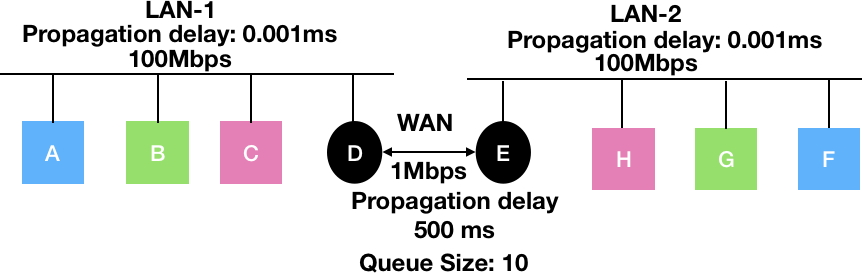
\includegraphics[scale=1.15]{src/Figures/chap2/chap2-fig07.jpg}
\caption{Experimental study of TCP Fairness}\label{chap2-fig07}
\end{figure}

For an experimental study of TCP fairness, a network simulation experiment under NS2 simulator can be conducted. For simplicity, consider a network as shown in Figure~\ref{chap2-fig07}, consisting of two LANs connected by a WAN link. The LAN bandwidth is configured as 100Mbps with propagation delay of 0.001ms, and WAN bandwidth is configured to be 1Mbps with propagation delay of 500ms. Each LAN consists of 3 hosts and correspondingly, a TCP Connection is established on one to one basis i.e. A-F, B-G, C-H. The first connection A-F is started at time T=0s, connection B-G is started at time T=15s and ${\rm 3}^{\text{rd}}$ connection C-H is started at time T=30s. All the connections are configured to transmit as much data as they can  till the experiment is terminated at time T=150s. The initial value of slow start threshold (\textit{ssthreshold}) is configured as 50MSS. The program code details and steps to conduct the experiments are described in Exercise~\ref{chap2-exe04}. The behaviour of \textit{cwnd} value w.r.t. time, and corresponding AIMD behaviour for each of the 3 connections is shown in Figure~\ref{chap2-fig08}. 

From the Figure~\ref{chap2-fig08}, it can be seen that when \textit{cwnd} reaches 50, network (WAN Link) witnesses congestion resulting in packet drops . Thus, \textit{cwnd} becomes 25, but network still remain severely congested (because earlier packets continue to remain in the network) which results in complete packet loss and \textit{ssthreshold} is set to 12 (half of 25.) and \textit{cwnd} starts from 1. For connection A-F (red color), connection starts time T=0s, and AIMD behaviour begins at about 14s and from then on follows saw tooth pattern. For connection B-G (green color), the connection starts at 15s, follows AIMD behaviour from T=29s. For connection C-H (blue color), connection starts at time 30s, and follows AIMD behaviour from T=44s. AIMD behaviour of ${\rm 2}^{\text{nd}}$ (B-G) and ${\rm 3}^{\text{rd}}$ connection (C-H) behaviour coincides with each other at about T=87s follows saw tooth pattern with \textit{cwnd} value varying between 18 and 35. AIMD behaviors of all 3 connections coincide at T=124s. Thus, the experimental simulation shows that TCP shares the WAN bandwidth among all 3 connections fairly from T=124s onwards.

\begin{figure}[H]
\centering
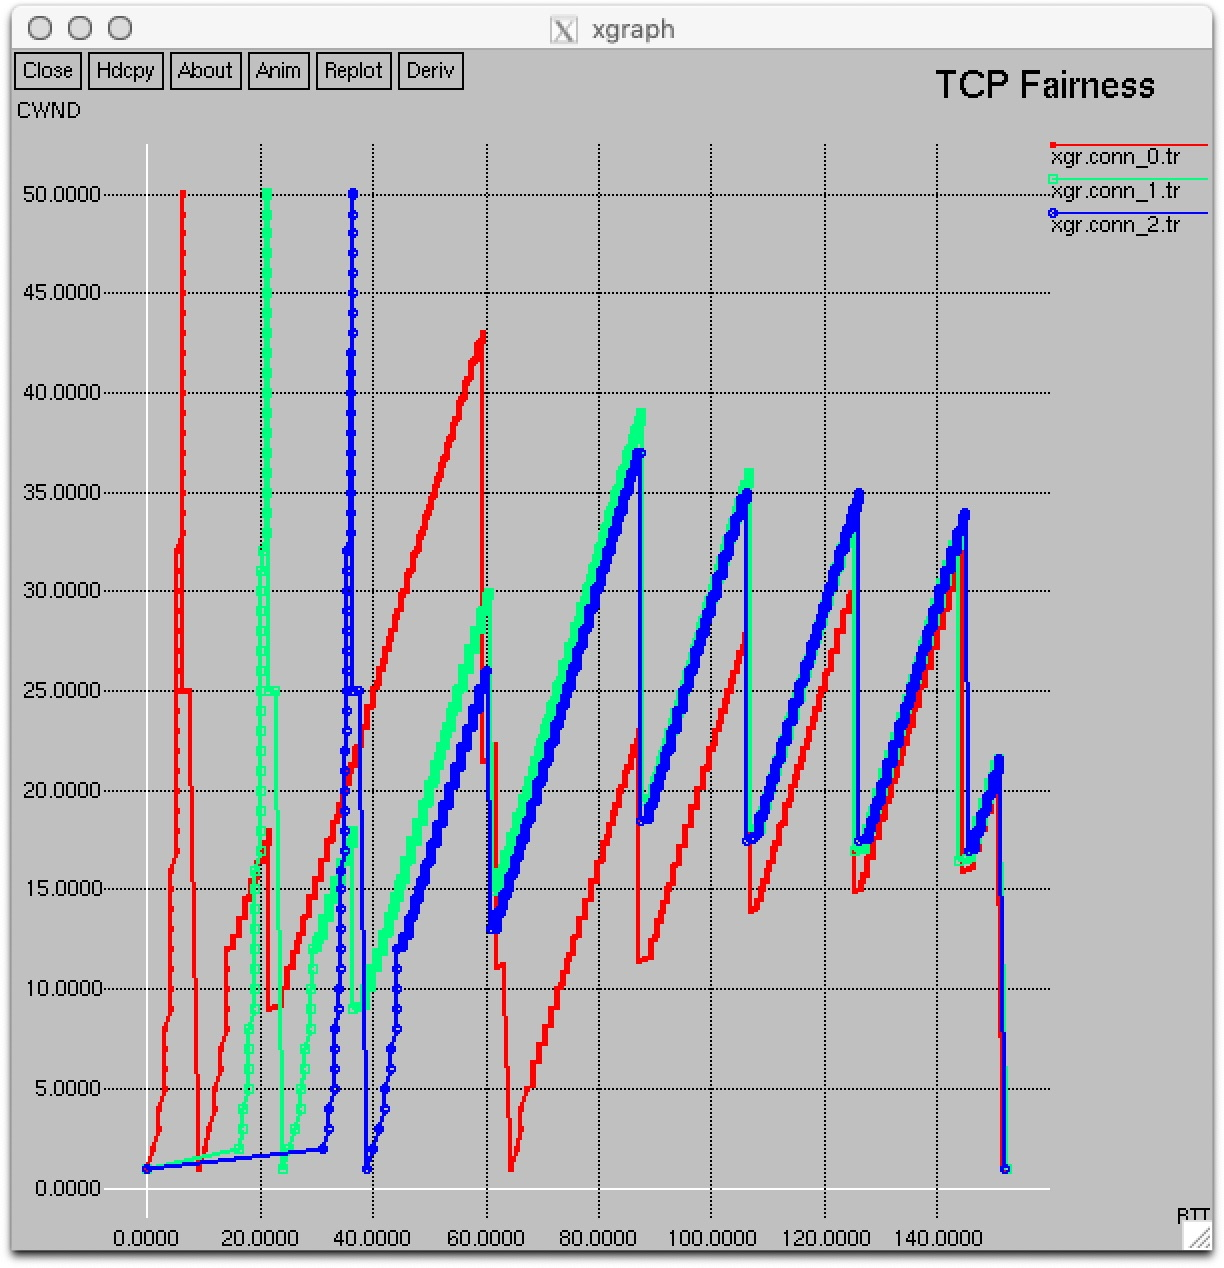
\includegraphics[scale=.85]{src/Figures/chap2/chap2-fig08.jpg}
\caption{TCP fairness behaviour among 3 connections}\label{chap2-fig08}
\end{figure}

\section*{Summary}

We have discussed the behaviour of TCP protocol when faced with network congestion. The congestion control mechanism of TCP is divided into 3 phases, namely a) Slow Start phase, b) Congestion Avoidance phase, and c) Fast Recovery phase. The transition between these phases is shown in Figure~\ref{chap2-fig04}. We also discussed that TCP is able to differentiate between mild congestion and severe congestion, accordingly  the recovery mechanism used. TCP is designed to perform optimally for long duration connection, continues to probe the network for optimal bandwidth and tries to maximize its throughput. Further, TCP congestion control algorithm follows AIMD behaviour, which also ensures that TCP is fair to all connections using a shared link. Experiential exercises have been provided so that reader can carry out these to develop better and realistic understanding of TCP congestion control algorithms.

\section*{Experiential Exercises}

All the experimental exercises are carried out using NS2 simulator (ns2) version 2.35 \cite{art2-key09}, Network Animator (nam) \cite{art2-key10}, and Xgraph 2D Plotter \cite{art2-key11}. This simulation experiments are used; mainly because in today’s computer system, TCP protocol implementation is optimized and uses TCP-Cubic Congestion control algorithm for congestion control where \textit{cwnd} does not start from value of 1, but some other higher value. Though Linux system allows changing congestion control algorithm to TCP-Reno, It is practically challenging to configure the other related tuning parameters (requires a detailed understanding of how these parameters work together, which is beyond the scope of this article). The instructions for installing NS2 and associated tools are given in Appendix. In additional to these experimental exercises, interactive animation are also available at \cite{art2-key14}.

To work on the simulation experiments, download the programs from \cite{art2-key12}, e.g. in a terminal window of the machine where \textit{NS2, Nam} and \textit{Xgraph} are installed, use the following command to download.
 
 \$ git clone \url{https://github.com/rprustagi/EL-TCP-Congestion-Control.git}

\setcounter{section}{0}
\section{Exercise}\label{chap2-exe01}

\textbf{Topic: Slow Start phase}

\begin{itemize}

\item[a.] Take the ns2 program \texttt{simpletcp.tcl} in \cite{art2-key12}.

\item[b.] This network simulation corresponds to two machines connected by a (duplex) link of bandwidth=1Mbps and propagation delay of 100ms as defined by following line (at line number 33). If desired, change the bandwidth and propagation delay by editing the values 

\texttt{\$ns duplex-link \$n1 \$n2 1Mb 100ms DropTail}

\item[c.] The program is designed to send FTP traffic which uses TCP as underlying protocol starting time T=0s till T=2.0s.

\item[d.] Invoke the simulator to run the program e.g.

\texttt{ns simpletcp.tcl}

\item[e.] The program will generate three output files, namely \texttt{“simpletcp.nam”} and \texttt{“simpletcp.tr”}, and \texttt{“tcpcong.tr”}. The first file \texttt{“simpletcp.nam”} is for viewing the FTP traffic transmission and TCP ack packets. The file \texttt{simpletcp.tr} contains ns2 events indicates when a packet is queued, dequeued and received etc. The file \texttt{tcpcong.tr} contains information about \textit{cwnd} adjustment with the progress of time. To view the animation, invoke the following command, and when animation windows open, click on play button.

\texttt{nam simpletcp.nam}

\item[f.] The animation will show first 1 packet being transmitted corresponding to \textit{cwnd}=1. When its ack is received, \textit{cwnd} is doubled and becomes 2 and thus 2 packets are transmitted. After both the \textit{acks} are received, \textit{cwnd} is doubled to 4, and 4 packets are transmitted. Continued in this way \textit{cwnd} becomes 8, then 16 and then becomes 20 (\textit{ssthreshold} limit).

\item[g.] To look at the growth of cwnd, we process the \texttt{tcpcong.tr} to generate time(x-axis) and cwnd (y-axis) event data as follows and plot the graph \cite{art2-key15} which shows the growth of cwnd in slow start phase.

\texttt{\$  awk -f cong.awk simpletcp.tr $>$xgr.tcp}

\texttt{\$ xgraph -lw 3 -m -x RTT -y CWND -t ``Slow Start" xgr.tcp}
\end{itemize}

\section{Exercise}\label{chap2-exe02}

\textbf{Topic: Congestion Avoidance phase}
\begin{itemize}

\item[a.] Repeat the steps of Exercise~\ref{chap2-exe01} with different value of window\_ (line 40) in \textit{tcl} file \texttt{“simpletcp.tcl”}, to configure the \textit{ssthreshold} value.

\item[b.] Run the ns2 simulator and plot the graphs and verify  exponential increase of \textit{cwnd} till it reaches the threshold value (defined by window\_) and after that it increases linearly.
\end{itemize}

\section{Exercise}\label{chap2-exe03}

\textbf{Topic: AIMD behaviour.}

\begin{itemize}

\item[a.] Consider the file \texttt{“tcpcong.tcl”} which simulates a network of 2 ethernet LANs connected via a WAN link of 1Mbps with propagation delay of 500ms. The LAN bandwidth is configured as 100Mbps with propagation delay of 0.001ms. The network topology for this simulated network is as shown in Figure~\ref{chap2-fig07}.

\item[b.] The experiment simulates 3 TCP connections, first one starting 0s, ${\rm 2}^{\text{nd}}$ one stating at 15s and ${\rm 3}^{\text{rd}}$ one starting at 30s. This starting time gap is configured with set conngap 15 (line number 20).

\item[c.] When simulation experiment is run i.e. \texttt{ns tcpcong.tcl}, it creates one events trace file \texttt{“tcpcong.tr”}, one animation events file \texttt{“tcpcong.nam”} and 3 TCP trace files corresponding to 3 TCP connections, named as \texttt{“conn\_0.tr”}, \texttt{conn\_1.tr“conn\_1.tr”}, and \texttt{conn\_2.tr}. These TCP trace files contain event details when such as change of \textit{cwnd} value, receiving duplicate ack and new TCP sequence number.

\item[d.] Extract timing events for \textit{cwnd} from one of the trace file, for example from \texttt{conn\_2.tr}

\texttt{\$awk -f cong.awk conn\_2.tr $>$xgr.conn2}

\texttt{\$xgraph -lw 3 -m -x Time -y CWND -t ``AIMD” xgr.conn2}

\item[e.] Plot the graph for the \textit{cwnd} change w.r.t. \textit{time}. The graph will be similar to as shown in Figure~\ref{chap2-fig05}.

\item[f.] Repeat the experiment with different initial values of \textit{ssthreshold} i.e. by changing value of configuration parameter window\_, and WAN link bandwidth, WAN link queue size to study the AIMD behaviour with different combinations.
\end{itemize}

\section{Exercise}\label{chap2-exe04}

\textbf{Topic: TCP Fairness.}

\begin{itemize}

\item[a.] Repeat the steps of Exercise~\ref{chap2-exe03}.

\item[b.] Extract timing events for cwnd from all of the TCP connection trace files such that x axis reflects time and y-axis reflects cwnd value.

\texttt{\$awk -f cong.awk conn\_0.tr $>$xgr.conn0}

\texttt{\$awk -f cong.awk conn\_1.tr $>$xgr.conn1}

\texttt{\$awk -f cong.awk conn\_2.tr $>$xgr.conn2}

\item[c.] Plot the graph for 3 TCP connections and study their AIMD Behaviour.

\texttt{\$xgraph -lw 3 -m -x Time -y CWND -t ``AIMD” xgr.conn0 xgr.conn1 xgr.conn2}

\end{itemize}

\section*{Appendix}

\noindent
\textbf{Setting up NS2, Nam and Xgraph on Ubuntu Linux.}

\begin{enumerate}[i.]

\item Installing Network Simulator NS-2. On a Ubuntu Linux

  \begin{itemize}
   \item[a.] The simplest way to install ns2 is using Linux install/upgrade install utility
   
   \texttt{sudo apt install ns2}

  \item[b.] To install from the source, download the code base from \cite{art2-key09} and follow the instructions to install the same.
  \end{itemize}

\item Installing Network Animator (nam)
      
      \begin{itemize}
   \item[a.] The simplest way to install nam is
   
   \texttt{sudo apt install nam}
   
   \item[b.] Alternatively, download the source code from \cite{art2-key10} and follow the instructions to install it.
   
   \end{itemize}

\item Installing Xgraph


\begin{itemize}
   \item[a.] Install xgraph \cite{art2-key11} \cite{art2-key15} using linux install utility
   
   \texttt{sudo apt install xgraph}
   
   \end{itemize}

\end{enumerate}

\vskip -1.3cm

\hfill\raisebox{-.1cm}{\includegraphics[scale=.9]{src/Figures/circledC.eps}}

\begin{thebibliography}{99}
\bibitem{art2-key01} Ram Rustagi, Viraj Kumar, “Understanding TCP Flow Control”, ACCS journal of Computing and Communications, Vol 3, Issue 2, June 2019,

 \url{https://journal.accsindia.org/experiential-learning-of-networking-technologies-understanding-tcp-flow-control/}, last accessed Aug 2019.

\bibitem{art2-key02}  RFC 793, “Transmission Control Protocol “, Information Sciences Institute, USC, CA, Sep 1981,

\url{https://tools.ietf.org/html/rfc793.}, Last accessed May 2019.

\bibitem{art2-key03} Kurose, Ross, “Computer Networking: A Top Down Approach”, section 3.5.5, ${\rm 6}^{\text{th}}$ edition, Pearson, 

\bibitem{art2-key04} \url{http://www.cs.binghamton.edu/~nael/cs428-528/deeper/jacobson-congestion.pdf}

\bibitem{art2-key05} RFC 5681, “TCP Congestion Control”, Allman, Paxson, Blanton; Sep 2009,

\url{https://tools.ietf.org/html/rfc5681,}  last accessed Aug 2019

\bibitem{art2-key06}RFC 3390, “Increasing TCP’s Initial Window”, Allman(NASA), Floyd(ICIR), Partridge (BBN Technologies), October 2002,

 \url{https://tools.ietf.org/html/rfc3390}, last accessed Aug 2019

\bibitem{art2-key07}  RFC 6928, “Increasing TCP’s Initial Window”, Chu, Dukkipati, Cheng, Mathis; Apr 2013, 

 \url{https://tools.ietf.org/html/rfc6928}, last accessed Aug 2019.

\bibitem{art2-key08} TCP Cubic: A TCP Friendly High Speed TCP Variant, {Ha, Rhee} North Carolina State Univ, Xu (Univ of Nebraska),

\url{https://www.cs.princeton.edu/courses/archive/fall16/cos561/papers/Cubic08.pdf}, last accessed Aug 2019.

\bibitem{art2-key09} The Network Simulator - ns-2,

\url{https://www.isi.edu/nsnam/ns/}, last accessed Aug 2019.

\bibitem{art2-key10} Nam: Network Animator,

\url{ https://www.isi.edu/nsnam/nam/}, last accessed Aug 2019.

\bibitem{art2-key11} Xgraph: General Purpose 2-D Plotter, 

\url{http://www.xgraph.org/index.html}, last accessed Aug 2019.

\bibitem{art2-key12} Experimental exercises and program code and sample results, 

\url{https://github.com/rprustagi/EL-TCP-Congestion-Control.git}. Last accessed Aug 2019.

\bibitem{art2-key13} Ram Rustagi, Viraj Kumar, “Understanding Basics of Transport Layer”, ACCS journal of Computing and Communications, Vol 2, Issue 3, September 2018 

\url{https://journal.accsindia.org/experiential-learning-of-networking-technologies-understanding-transport-layer-basics/}, last accessed Aug 2019

\bibitem{art2-key14} Understanding TCP Congestion Control with interactive animations,

\url{https://media.pearsoncmg.com/aw/ecs\_kurose\_compnetwork\_7/cw/content/interactiveanimations/tcp-congestion/index.html,} last accessed May 2019.

\bibitem{art2-key15} Using Options with Xgraph when plotting results,

\url{https://ns2blogger.blogspot.com/p/plotting-results-on-xgraph.html}. last accessed Aug 2019.

\end{thebibliography}
\end{multicols}



%~ \noindent
%~ \begin{tabular}{V{2.5}cp{14.2cm}V{2.5}}
%~ \clineB{1-2}{2.5}
 %~ &\\
%~ \raisebox{-4cm}{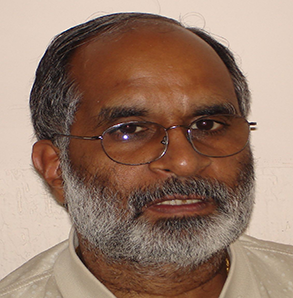
\includegraphics{src/Figures/authors/Rustagi_RPR-PP-Photo.png}} & 

%~ \centerline{\large\bf Prof. Ram P. Rustagi}

%~ \bigskip
%~ Dr.~Ram P. Rustagi is currently working as Professor, CSE dept, KSIT Bangalore, and honed up his academic skills with Ph.D from IIT Delhi, and M.Tech from IISc Bangalore. Prior to KSIT, at Cavisson Systems, he mentored new technology development using Machine Learning techniques in Security and Performance Monitoring. At PES University, he had taught Undergraduates, Post Graduates students, and successfully guided 3 Ph.D scholars. At PESU, he brought innovations in teaching computer network and security courses, and introduced practical experiential learning exercises.\\
%~ &\\  
%~ \raisebox{-3.7cm}{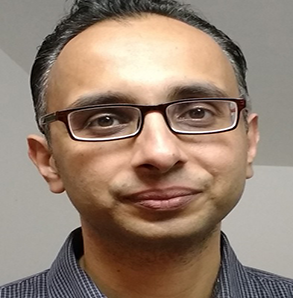
\includegraphics{src/Figures/authors/Viraj_Kumar.png}} & 

%~ \centerline{\large\bf Prof. Viraj Kumar}

%~ \bigskip
%~ Dr.~Viraj Kumar is a Visiting Professor at the Divecha Centre for Climate Change, IISc Bangalore and the Vice-Chair of ACM India’s Special Interest Group in Computer Science Education (iSIGCSE). He was a consultant to the Committee to draft the National Education Policy (2017-18), and contributed to two education-related task groups of the Karnataka Knowledge Commission (2014-16). He holds a PhD in Computer Science from the University of Illinois at Urbana-Champaign.\\
%~ &\\
%~ \clineB{1-2}{2.5}
%~ \end{tabular}

%~ \vskip 1cm

%~ \begin{figure}[H]
%~ \centering
%~ 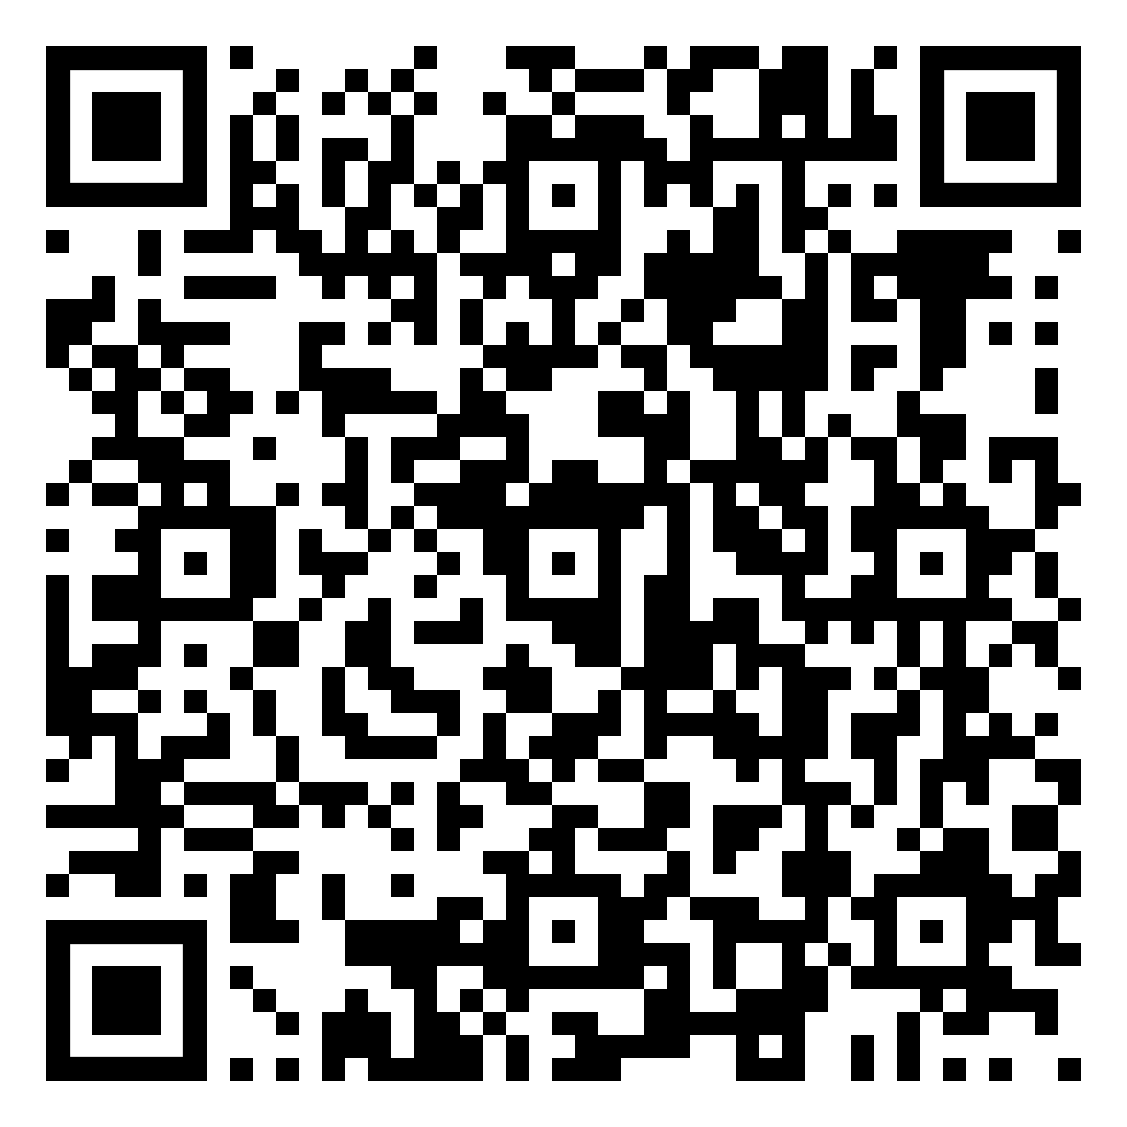
\includegraphics[scale=.15]{src/Figures/QR-codes/qr-code_experiential-learning.png}

%~ \medskip

%~ {\large\sf Access this article on the Web}
%~ \end{figure}


















